\documentclass[10pt]{article}

\usepackage{polski}
\usepackage{tabularx}
\usepackage{graphicx}
\usepackage{hyperref}
\usepackage{subfigure}
\usepackage[font=footnotesize]{caption}
\usepackage{geometry}
% \usepackage{indentfirst}
\usepackage{amsmath}
\usepackage{fancyhdr}

\newcolumntype{C}[1]{>{\centering\let\newline\\\arraybackslash\hspace{0pt}}m{#1}}

\captionsetup{hypcap=false}
\graphicspath{{images/}}
\newgeometry{tmargin=4cm, bmargin=4cm, lmargin=3.2cm, rmargin=3.2cm}
\pagestyle{fancy}
\def\nl{\\\hline}

\begin{document}
\begin{titlepage}
  \begin{center}
    \LARGE \textsc{Politechnika Wrocławska}\\
    \vspace*{0.2cm}
    \Large \textsc{Wydział Informatyki i Telekomunikacji}\\
    \vspace*{0.4cm}
    
\includegraphics[width=0.2\textwidth]{figures/WITlogo.png}\\
    \vspace*{0.2cm}
    \vspace*{2cm}

    \centerline{\rule{\textwidth}{1.2pt}}
    \vspace{0.4cm}
    \Huge\textbf{Systemy inteligentne}
    \centerline{\rule{\textwidth}{1.2pt}}
    \vspace{1cm}
    \LARGE Sprawozdanie z projektu\\
    \vspace{3.5cm}
    \textsc{Autorzy}\\
    \vspace{0.2cm}
    \textbf{Przemysław Barcicki, 260324}\\
    \vspace{0.1cm}
    \textbf{Dominik Lenio, 260274}\\
    \vspace{0.1cm}
    kierunek: \textbf{Inżynieria systemów}

    \vspace*{\fill}
    \Large \textit{30 maja 2023}

  \end{center}
\end{titlepage}

\begin{abstract}
  W ramach projektu przeprowadzono porównanie skuteczności algorytmów min-max oraz min-max z żalem w celu znalezienia najkrószej ścieżki między dwoma wierzchołkami w grafie nieskierowanym, gdzie długość krawędzi podana jest jako możliwy zakres w postaci rozkładu równomiernego. Algorytm podczas szukania najlepszej ścieżki ma wgląd tylko w informację o minimum i maksimum z rozkładu.
\end{abstract}

\section{Wstęp -- opis problemu}
\label{sec:wstep}
Optymalizacja jest aktualnie dziedziną na której polega cały świat. Pozwala ona na przykładowo minimalizację kosztów prowadzenia działalności poprzez lepszy dobór dostawców czy też zmniejszanie czasu potrzebnego na wykonanie skomplikowanych procesów poprzez ich lepsze kolejkowanie. Znalezienie dobrego sposobu na optymalizację danego procesu, w szczególności w zmiennych warunkach, może mówić o istnieniu danego podmiotu na rynku.

Optymalizacja procesów w przypadku gdzie dany proces ma z góry określone zmienne nie jest żadnym problemem. Istnieje bardzo dużo różnych algrytmów dla różnych problemów które bardzo dobrze sobie radzą z optymalizacją takich zadań. Problem pojawia się jednak gdy w optymalizacji mamy do czynienia ze zmienną, która może przyjąć pewien zakres wartości. Gotowe algorytmy mogą radzić sobie z szukaniem takich rozwiązań, ale w żaden sposób nie korzystamy z informacji o szerokości rozkładu, co może przekładać się na gorsze wyniki.

Celem sprawozdania jest przeprowadzenie analizy oraz opisanie wyników działania algorytmów min-max oraz min-max regret dla problemu szukania ścieżki pomiędzy dwoma wierzchołkami w nieskierowanym grafie, gdzie długości krawędzi dane są w postaci możliwych zakresów dodatnich wartości przedstawiających rozkład równomierny.

\section{Definicja problemu}
Znając aktualny scenariusz $s \in S$ określony za pomocą informacji o nieskierowanym grafie wejściowym $G = (V, E)$ oraz zakresach odległości
\begin{eqnarray*}
  s = E \rightarrow \left\{e \in (o^-,  o^+): 0 < o^- \leq o^+ < \infty\right\},
\end{eqnarray*}

szukamy takiego rozwiązania $x = \left(e_1, e_2, \dots, e_n\right)$, $x \in X$ które będzie minimalizować długość trasy od źródła do celu, $v_{start}$ do $v_{koniec}$, którą możemy zdefiniować jako:
\begin{equation}
  \min_{e \in x} \sum_{i=1}^{n} s_x,
\end{equation}

Korzystając z tych definicji możemy okreslić dwa różne podejścia optymalizacyjne, jedno klasyczne korzystające z samej informacji o aktualnej trasie oraz drugie, korzystające z funkcji żalu do określenia najlepszej trasy.

\subsection{Min-max}
Dla danego rozwiązania $x \in X$ i danego scenariusza $s \in S$ możemy określić pewną funkcję $val(x, s)$ oceniającą jak dobre jest dane rozwiązanie. Funckja ta będzie sumą pewnej długości opisującej daną ścieżkę. Dla danej trasy możemy rozpatrywać trzy różne wartości, są to: wartość oczekiwana danej trasy, teoretycznie minimalna i teoretycznie maksymalna długość trasy.

\begin{eqnarray}
  {val}^\sim(x, s) = \sum_{e \in x}& \frac{1}{2}\left(s_e^+ +  s_e^-\right), \\
  {val}^+(x, s) =    \sum_{e \in x}& s_e^+, \\
  {val}^-(x, s) =    \sum_{e \in x}& s_e^-
\end{eqnarray}
\begin{equation}
  \min_{x \in X} \max_{s \in S} val(x, s)
\end{equation}

\subsection{Min-max regret}
Metoda min-max z żalem jest bardzo podobna do tej metody bez. Różnica to wprowadzenie pewnego dodatkowego elementu określanego jako żal $val^*_s$, który zamienia nam wartość liczonej funkcji z samej odległości między wierzchołkami na odchylenie od najlepszego możliwego rozwiązania dla danego scenariusza, definiowanej jako optymalne rozwiązanie w scenariuszu $s$.

Bardzo często zdarza się sytuacja, że samo określenie teoretycznie najlepszej ścieżki jest bardzo trudne, więc w praktyce często korzysta się w tym miejscu z pewnego oszacowania, najczęściej z relaksacji. W przypadku małych grafów $|E| \ll 50$ w celu znalezienia najlepszej wartości można wykonać przegląd zupełny.

\begin{equation}
  \min_{x \in X} \max_{s \in S} val(x, s) - val^*_s
\end{equation}

\subsection{Przykład}
Rozpatrzmy prosty przykład aby zobrazować różnice między każdym z podejść. Do tego celu skorzystajmy z prostego grafu znajdującego się na rysunku (\ref{fig:example}), gdzie na każdej z krawędzi zaznaczono możliwe rozkłady.
\begin{center}
  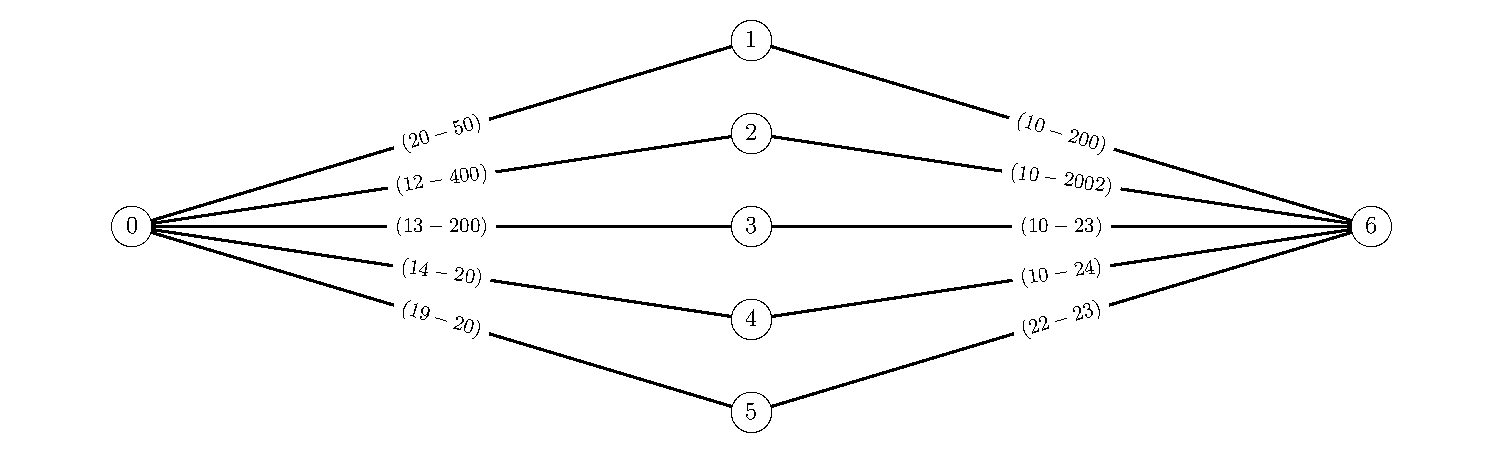
\includegraphics[width=\linewidth]{figures/example.pdf}
  \captionof{figure}{Przykładowy graf gdzie wierzchołek 0 to $v_{start}$, a wierzchołek 6 to $v_{koniec}$}
  \label{fig:example}
\end{center}

Podejście bez żalu, w zależności od rozpatrywanej metody w przypadku tego grafu będzie zachowywało się różnie. Ścieżki wygenerowane przez każdą z metod znajdują się w tabeli (\ref{tab:example_paths})
\begin{center}
  \captionof{table}{Tabela zawierająca ścieżki, wartości funkcji $val(x, s)$, minimum oraz maksimum dla każdej z metod}
  \begin{tabular}{|c|c|c|c|c|}
    \hline
    $f$          & Ścieżka   & $f(x)$ & min & max  \\ \hline
    ${val}^\sim$ & (0, 4, 6) & 34     & 24  & 44   \\ \hline
    ${val}^-$    & (0, 2, 6) & 22     & 22  & 2402 \\ \hline
    ${val}^+$    & (0, 5, 6) & 43     & 41  & 43   \\ \hline \hline
    $val^*_s$    & (0, 4, 6) & 14     & 24  & 44   \\ \hline
  \end{tabular}
  \label{tab:example_paths}
\end{center}
Nawet na tak prostym przykładzie widać pewne różnice, każdego z tych podejść. Szukanie po wartości minimalnej, może wpaść w takie rozwiązanie, w którym może i minimalna wartość ścieżki jest bardzo niska, ale wartość w najgorszym wypadku może mieć bardzo słabe konsekwencje. Tak samo dla przypadku z szukaniem po najgorszym możliwym przypadku. Przyjmowanie każdego rozwiązania, pod warunkiem że wartość maksymalna lekko spada może sprawić, że wartość minimalna może być bardzo wysoka co również może skutkować słabym rzeczywistym wynikiem.

W tym przypadku, optymalizowanie po wartości oczekiwanej ścieżki jak i po wartości pochodzącej z funkcji żalu daje takie same wyniki, widać pewną różnice w ich zachowaniu po samej wartości funkcji, co może nam sugerować, że dla większych przypadków rozwiązania na które te podejścia wskazują, mogą być zgoła inne.

\section{Badania}
Analizę przeprowadzono na dwóch obszarach, w pierwszym z nich skorzystano z przeglądu zupełnego dla małych grafów $|E| < 40$, w drugim $|E| < 1000$. W drugim pojdeściu skorzystano z pewnej heurestyki, w której przeglądano tylko część wszystkich możliwych rozwiązań w celu optymalizacji, które zostały wcześniej wybrane jako quasioptymalne. W dużych grafach tylko takie podejście jest możliwe, ze względu na wysoką złożoność czasową algorytmów potrzebnych do policzenia każdej możliwej ścieżki w każdym możliwym scenariuszu.

Każdy wygenerowany graf stworzony jest na zasadzie pierścienia, gdzie każdy wierzchołek połączony jest z $K$ sąsiadami po jego "prawej" i "lewej" stronie ($|E| = K \times |V|$), a początek i koniec trasy, znajdują się po wzajemnej przekątnej tak aby wszystkie najkrótsze trasy w ilościach krawędzi były sobie równe, ale zawsze była ewentualna możliwość przeskoku do następnego wierzchołka inną trasą. Wygenerowane długości pomiędzy każdym z wierzchołków pochodzą z rozkładu równomiernego ($\left(o^-,  o^+\right);\ 0 < o^- < o^+ < P$) i dla każdego nowego grafu są generowane od nowa. Każdy z grafów można opisać tymi trzema wartościami $G \leftarrow (K, |V|, P)$.

\subsection{Przegląd zupełny}
W tabeli (\ref{tab:all}) pokazano wyniki przeglądu zupełnego dla grafów z 10, 12, 14, 16, 18 i 20 wierzchołkami dla grafów $(2, x, 1)$.
\filbreak
\begin{center}
  \captionof{table}{Tabela zawierająca minimum oraz maksimum dla każdej z metod w danym grafie.}
  \begin{tabular}{|C{0.08\linewidth}|C{0.08\linewidth}|C{0.08\linewidth}|C{0.08\linewidth}|}
    \hline
    \multicolumn{3}{|c|}{$G \rightarrow \left(2, 10, 1\right)$} \\ \hline
    $f$          & min  & max   \\ \hline
    $val^*_s$    & 0.43 & 2.33  \\ \hline
    ${val}^-$    & 0.43 & 2.33  \\ \hline
    ${val}^+$    & 0.6  & 1.66  \\ \hline
    ${val}^\sim$ & 0.6  & 1.66  \\ \hline
  \end{tabular}
  \begin{tabular}{|C{0.08\linewidth}|C{0.08\linewidth}|C{0.08\linewidth}|C{0.08\linewidth}|}
    \hline
    \multicolumn{3}{|c|}{$G \rightarrow \left(2, 12, 1\right)$} \\ \hline
    $f$          & min  & max  \\ \hline
    $val^*_s$    & 1.11 & 2.74 \\ \hline
    ${val}^-$    & 1.11 & 2.74 \\ \hline
    ${val}^+$    & 1.73 & 2.18 \\ \hline
    ${val}^\sim$ & 1.39 & 2.39 \\ \hline
  \end{tabular}
  \begin{tabular}{|C{0.08\linewidth}|C{0.08\linewidth}|C{0.08\linewidth}|C{0.08\linewidth}|}
    \hline
    \multicolumn{3}{|c|}{$G \rightarrow \left(2, 14, 1\right)$} \\ \hline
    $f$          & min  & max  \\ \hline
    $val^*_s$    & 0.74 & 3.26 \\ \hline
    ${val}^-$    & 0.74 & 3.26 \\ \hline
    ${val}^+$    & 1.5  & 2.52 \\ \hline
    ${val}^\sim$ & 0.8  & 3.12 \\ \hline
  \end{tabular}
  \begin{tabular}{|C{0.08\linewidth}|C{0.08\linewidth}|C{0.08\linewidth}|C{0.08\linewidth}|}
    \hline
    \multicolumn{3}{|c|}{$G \rightarrow \left(2, 16, 1\right)$} \\ \hline
    $f$          & min  & max  \\ \hline
    $val^*_s$    & 0.66 & 3.18 \\ \hline
    ${val}^-$    & 0.66 & 3.18 \\ \hline
    ${val}^+$    & 1.96 & 2.72 \\ \hline
    ${val}^\sim$ & 0.66 & 3.18 \\ \hline
  \end{tabular}
  \begin{tabular}{|C{0.08\linewidth}|C{0.08\linewidth}|C{0.08\linewidth}|C{0.08\linewidth}|}
    \hline
    \multicolumn{3}{|c|}{$G \rightarrow \left(2, 18, 1\right)$} \\ \hline
    $f$          & min  & max  \\ \hline
    $val^*_s$    & 1.34 & 2.57 \\ \hline
    ${val}^-$    & 1.34 & 2.57 \\ \hline
    ${val}^+$    & 1.34 & 2.57 \\ \hline
    ${val}^\sim$ & 1.34 & 2.57 \\ \hline
  \end{tabular}
  \begin{tabular}{|C{0.08\linewidth}|C{0.08\linewidth}|C{0.08\linewidth}|C{0.08\linewidth}|}
    \hline
    \multicolumn{3}{|c|}{$G \rightarrow \left(2, 20, 1\right)$} \\ \hline
    $f$          & min  & max  \\ \hline
    $val^*_s$    & 0.86 & 2.3  \\ \hline
    ${val}^-$    & 0.65 & 3.35 \\ \hline
    ${val}^+$    & 0.86 & 2.3  \\ \hline
    ${val}^\sim$ & 0.86 & 2.3  \\ \hline
  \end{tabular}
  \\\label{tab:all}
\end{center}
Zauważyć można, że w przypadku małych grafów rzadkich, gdzie jest mało najkrótszych ścieżek i nie jest wysoka różnica między najlepszym a najgorszym scenariuszem, optymalizacja za pomcą funkcji żalu daje takie same wyniki jak inne algorytmy.

\subsection{Heurestyka}
W metodzie heurestycznej wykorzystano dwa uproszczenia, które zdecydowanie skracają przeszukiwanie grafu, ale mogą nie znajdywać optymalnego rozwiązania, lecz inne do niego zbliżone. Oba tyczą się ograniczenia obszaru przeszukiwania i polegają na wcześniejszym wygenerowaniu mniejszej ilości scenariuszy do przeszukiwania i na ich podstawie wygenerowanie najkrótszych ścieżek, będzie się to objawiać szukaniem  W tabeli (\ref{tab:some}) zamieszczono wyniki przeszukiwania grafów z 50, 70, 90, 110, 130 i 150 wierzchołkami w kombinacji $(5, x, 5)$

\filbreak
\begin{center}
  \captionof{table}{Tabela zawierająca minimum oraz maksimum dla każdej z metod w danym grafie.}
  \begin{tabular}{|C{0.08\linewidth}|C{0.08\linewidth}|C{0.08\linewidth}|C{0.08\linewidth}|}
    \hline
    \multicolumn{3}{|c|}{$G \rightarrow \left(5, 50, 5\right)$} \\ \hline
    $f$          & min  & max   \\ \hline
    $val^*_s$    & 6.26 & 11.6  \\ \hline
    ${val}^-$    & 2.64 & 15.46 \\ \hline
    ${val}^+$    & 6.26 & 11.6  \\ \hline
    ${val}^\sim$ & 4.08 & 13.59 \\ \hline
  \end{tabular}
  \begin{tabular}{|C{0.08\linewidth}|C{0.08\linewidth}|C{0.08\linewidth}|C{0.08\linewidth}|}
    \hline
    \multicolumn{3}{|c|}{$G \rightarrow \left(5, 70, 5\right)$} \\ \hline
    $f$          & min  & max  \\ \hline
    $val^*_s$    & 5.46 & 14.24 \\ \hline
    ${val}^-$    & 3.73 & 18.56 \\ \hline
    ${val}^+$    & 6.83 & 13.2 \\ \hline
    ${val}^\sim$ & 4.56 & 14.83 \\ \hline
  \end{tabular}
  \begin{tabular}{|C{0.08\linewidth}|C{0.08\linewidth}|C{0.08\linewidth}|C{0.08\linewidth}|}
    \hline
    \multicolumn{3}{|c|}{$G \rightarrow \left(5, 90, 5\right)$} \\ \hline
    $f$          & min  & max  \\ \hline
    $val^*_s$    & 6.41 & 20.45 \\ \hline
    ${val}^-$    & 4.51 & 22.51 \\ \hline
    ${val}^+$    & 5.25 & 19.61 \\ \hline
    ${val}^\sim$ & 5.25 & 19.61 \\ \hline
  \end{tabular}
  \begin{tabular}{|C{0.08\linewidth}|C{0.08\linewidth}|C{0.08\linewidth}|C{0.08\linewidth}|}
    \hline
    \multicolumn{3}{|c|}{$G \rightarrow \left(5, 110, 5\right)$} \\ \hline
    $f$          & min  & max  \\ \hline
    $val^*_s$    & 8.03 & 27.52 \\ \hline
    ${val}^-$    & 4.68 & 41.38 \\ \hline
    ${val}^+$    & 13.4 & 24.31 \\ \hline
    ${val}^\sim$ & 8.92 & 26.24 \\ \hline
  \end{tabular}
  \begin{tabular}{|C{0.08\linewidth}|C{0.08\linewidth}|C{0.08\linewidth}|C{0.08\linewidth}|}
    \hline
    \multicolumn{3}{|c|}{$G \rightarrow \left(5, 130, 5\right)$} \\ \hline
    $f$          & min  & max  \\ \hline
    $val^*_s$    & 9.81 & 35.27 \\ \hline
    ${val}^-$    & 6.23 & 66.08 \\ \hline
    ${val}^+$    & 12.32 & 29.32 \\ \hline
    ${val}^\sim$ & 11.0 & 30.52 \\ \hline
  \end{tabular}
  \begin{tabular}{|C{0.08\linewidth}|C{0.08\linewidth}|C{0.08\linewidth}|C{0.08\linewidth}|}
    \hline
    \multicolumn{3}{|c|}{$G \rightarrow \left(5, 150, 5\right)$} \\ \hline
    $f$          & min  & max  \\ \hline
    $val^*_s$    & 11.78 & 36.32  \\ \hline
    ${val}^-$    & 7.54 & 67.79 \\ \hline
    ${val}^+$    & 13.77 & 31.9  \\ \hline
    ${val}^\sim$ & 10.52 & 33.3  \\ \hline
  \end{tabular}
  \\\label{tab:some}
\end{center}

\section{Wnioski}
Optymalizowanie za pomocą funkcji żalu pozwala nam minimalizować ewentualne złe skutki wybrania jednej metody względem drugiej, może być to potrzebne w przypadkach gdzie równie ważne są najgorsze i najlepsze możliwości tak jak np. w inwestowaniu czy bankowości gdzie każda możliwość jest niewiadomą. Zdarza się, że w pewnych warunkach znalezione rozwiązanie nie jest takie jakiego można się spodziewać i inne metody dorównują jakością, lecz nie mamy pewności w żadnej innej, że rozwiązanie które znajdziemy nie bierze pod uwage różnicy między najlepszym a najgorszym możliwym scenariuszem.

\newpage
\appendix

\section{Kod źródłowy}
Kody źródłowe umieszczone zostały w repozytorium GitHub:

\noindent \url{https://github.com/mlodybercik/nondeterministic-regret-path}.

\begin{thebibliography}{9}
    \bibitem{bib:minmax}
    Hassene Aissi, Cristina Bazgan, Daniel Vanderpooten.
    Min-max and min-max regret versions of some combinatorial optimization problems: a survey. (2007, ffhal-00158652)

    \bibitem{bib:tps_regret}
    Refael Hassin, Ariel Keinan
    Greedy Heuristics with Regret, with Application to the Cheapest Insertion Algorithm for the TSP

\end{thebibliography}

\end{document}